%Start
%
%
%******************************************************************************************************%
%                                  linear harmonic oscillator                                          %
%******************************************************************************************************%								 %
% Version 1,                                                                                           %
% 09.07.2023                                                                                           %
% L.Lentz@umwelt-campus.de                                                                             %
%******************************************************************************************************%
%
%
\documentclass[tikz,border=10pt]{standalone}
\usetikzlibrary{calc,intersections,backgrounds}
\usepackage{ifthen}
%
\tikzset{
axes/.style = {line width = 0.7pt},
grid/.style = {line width = 0.3pt,color = gray},
plots/.style = {samples=300,smooth,line width = 0.7pt}
}
%
\begin{document}
%
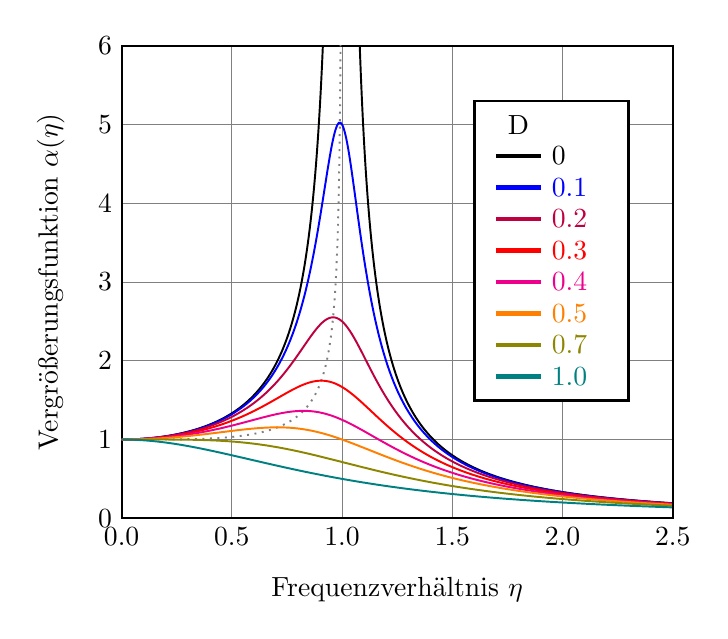
\begin{tikzpicture}
%
\def\width{7}
%
\def\Dlist{0,0.1,0.2,0.3,0.4,0.5,0.7,1.0}
\def\colorlist{{"black","blue","purple","red","magenta","orange","olive","teal"}}
\def\xlist{0.0,0.5,1.0,1.5,2.0,2.5}
\def\ampylist{0,1,2,3,4,5,6}
\def\phaseylist{0/0,-0.25*3.14/$-\frac{1}{4}\pi$,-0.5*3.14/$-\frac{1}{2}\pi$,-0.75*3.14/$-\frac{3}{4}\pi$,-3.14/$-\pi$}
%
\def\xmax{2.5}
\def\ymax{6}
\def\tagshift{0.9cm}
%
% scale x-axis to match width
\pgfmathsetmacro{\xsc}{\width/\xmax}
\begin{scope}[xscale=\xsc]
%
% x-grid and x-tick-labels
\foreach \x in \xlist {
\draw[grid](\x,0)--(\x,\ymax);
\node[anchor = north] at (\x,0){\x};
}
%
% y-grid and y-tick-labels
\foreach \y in \ampylist{\draw[grid](0,\y)--(\xmax,\y)node[at start, left, color = black]{\y};}
%
% Frames
\draw[axes](0,0)rectangle(\xmax,\ymax);
%
% Legend box
\draw[fill=white,draw=black,line width=1pt] (1.6,5.3) rectangle (2.3,1.5);
\node[] at (1.8,5){D};
%
%plot curves for D-values from list
\foreach \D [count=\i] in \Dlist {
%
	\pgfmathsetmacro{\c}{\colorlist[\i-1]} % get color 
	\draw[line width = 1.5pt,color=\c] (1.7,5-\i*0.4)--(1.9,5-\i*0.4)node[at end,right]{\D}; % legend entry
	%
	\begin{scope}
	\clip[](0,0) rectangle (\xmax,\ymax);% clip plot to frame
	\ifthenelse{\i=1}{\draw[domain=0.01:0.707,variable=\x,plots,color=gray,dotted] plot ({sqrt(1-2*\x^2)},{1/2*sqrt(1/(\x^2-\x^4))});};
	\ifthenelse{\lengthtest{\D pt = 0pt}}
		{
		\draw[domain=0:0.99,variable=\x,plots,color=\c] plot (\x,{sqrt(1/((2*\D*\x)^2+(1-\x^2)^2))});
		\draw[domain=1.01:\xmax,variable=\x,plots,color=\c] plot (\x,{sqrt(1/((2*\D*\x)^2+(1-\x^2)^2))});
		}
		{
		\draw[domain=0:\xmax,variable=\x,plots,color=\c] plot (\x,{sqrt(1/((2*\D*\x)^2+(1-\x^2)^2))});% plot amplitude magnification
		}
	\end{scope}
	%
%
}
% axis labels
\node[rotate=90] at($(0,\ymax/2)+(-\tagshift/\xsc,0)$){Vergrößerungsfunktion $\alpha(\eta)$};
\node[] at($(\xmax/2,0)+(0,-\tagshift)$){Frequenzverhältnis $\eta$};
%
\end{scope}
%
\end{tikzpicture}
%
\end{document}
%
%
%Ende